\section{Performance Degradation} \label{sec:performance-degradation}

\begin{frame}{Performance Degradation}
    
    We evaluated four distinct statistic models:
    
    \small
    \begin{itemize}
        \item \textbf{Random Forest}: An ensemble method combining multiple decision trees, where final prediction is determined by majority voting
        \item \textbf{Gradient Boosting}: Sequential ensemble approach that iteratively improves predictions by combining weak learners (in our case decision trees)
        \item \textbf{XGBoost}: Advanced implementation of gradient boosting with enhanced regularization and computational efficiency
        \item \textbf{Logistic Regression}: \textcolor{gray}{[baseline]} Classic linear classifier used as a reference model
    \end{itemize}
    
\end{frame}

\begin{frame}{Fine Tuning and Performance Metric}

    \textbf{Performance Metric}

    We used the \textbf{Area Under the Receiver Operating Characteristic Curve (ROC-AUC)} as the performance metric for our models.
    
    \textbf{Fine Tuning}

    We performed a \textbf{hyperparameter tuning} using the \textbf{Grid Search} method with 5-fold cross-validation.

    \begin{adjustbox}{margin=-0.5em 0em}
    \begin{columns}[T,totalwidth=\textwidth]
        \begin{column}{0.38\textwidth}
            \centering
            \textbf{Random Forest}
            \vskip 0.5em
            {\scriptsize
            \begin{tabular}{|l|c|}
            \hline
            \textbf{Params} & \textbf{Value} \\
            \hline
            n\_estimators & 125 \\
            max\_depth & 5 \\
            min\_samples\_split & 5 \\
            min\_samples\_leaf & 1 \\
            bootstrap & True \\
            \hline
            \end{tabular}
            }
        \end{column}
        \begin{column}{0.34\textwidth}
            \centering
            \textbf{Gradient Boosting}
            \vskip 0.3em
            {\scriptsize
            \begin{tabular}{|l|c|}
            \hline
            \textbf{Params} & \textbf{Values} \\
            \hline
            n\_estimators & 500 \\
            max\_depth & 3 \\
            learning\_rate & 0.005 \\
            subsample & 0.4 \\
            \hline
            \end{tabular}
            }
        \end{column}
        \begin{column}{0.29\textwidth}
            \centering
            \textbf{XGBoost}
            \vskip 0.5em
            {\scriptsize
            \begin{tabular}{|l|c|}
            \hline
            \textbf{Params} & \textbf{Values} \\
            \hline
            n\_estimators & 100 \\
            max\_depth & 6 \\
            learning\_rate & 0.1 \\
            subsample & 0.7 \\
            gamma & 5 \\
            \hline
            \end{tabular}
            }
        \end{column}
    \end{columns}
    \end{adjustbox}

\end{frame}

\begin{frame}%{Performance Comparison}

    \vspace{1em}

    \begin{columns}
        \begin{column}{0.5\textwidth}
            \begin{figure}
                \centering
                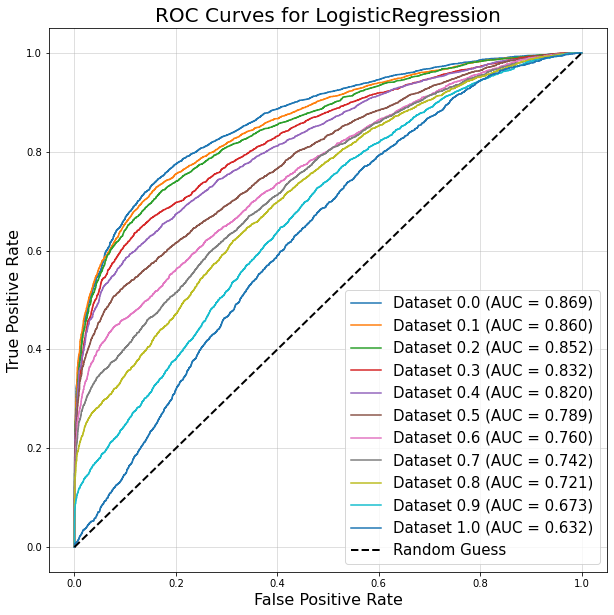
\includegraphics[width=\textwidth]{lr_auc.png}
                \vskip 0.6em
                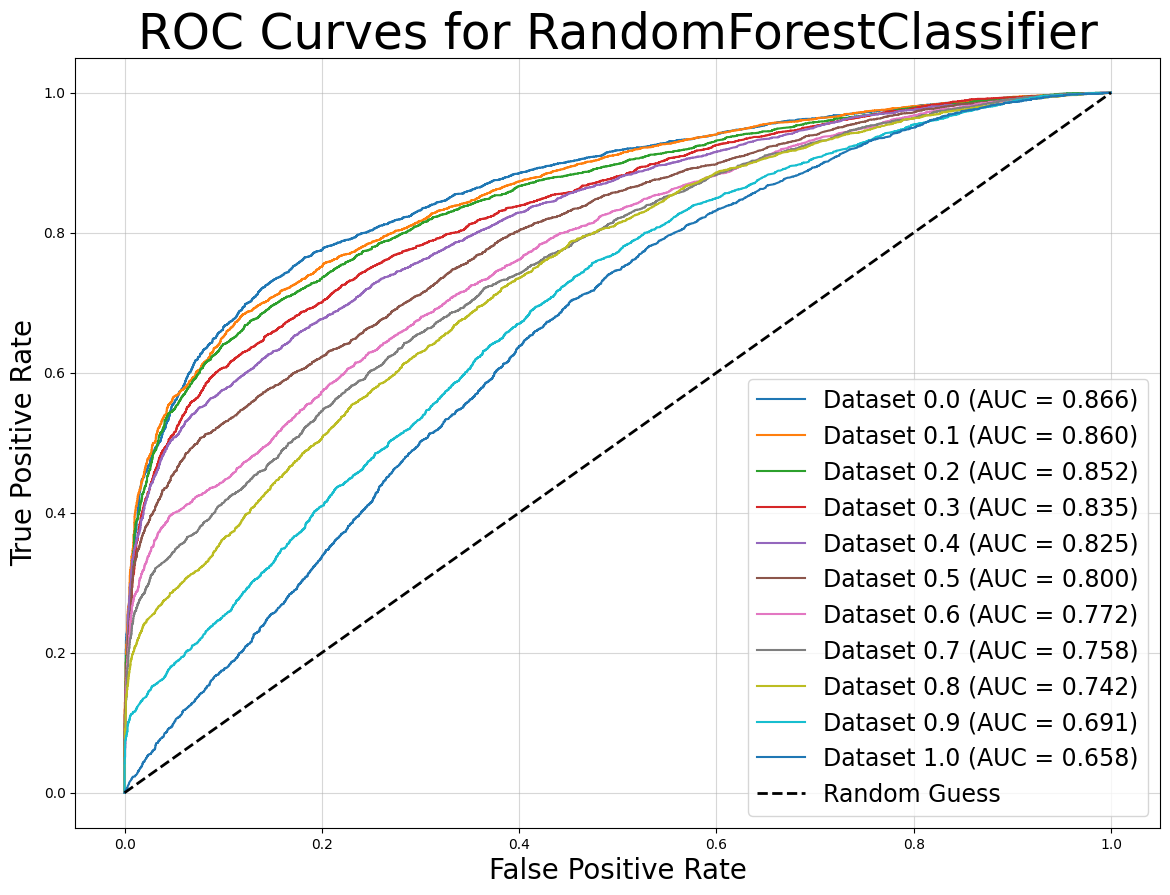
\includegraphics[width=\textwidth]{rf_auc.png}
            \end{figure}
        \end{column}
        \begin{column}{0.5\textwidth}
            \begin{figure}
                \centering
                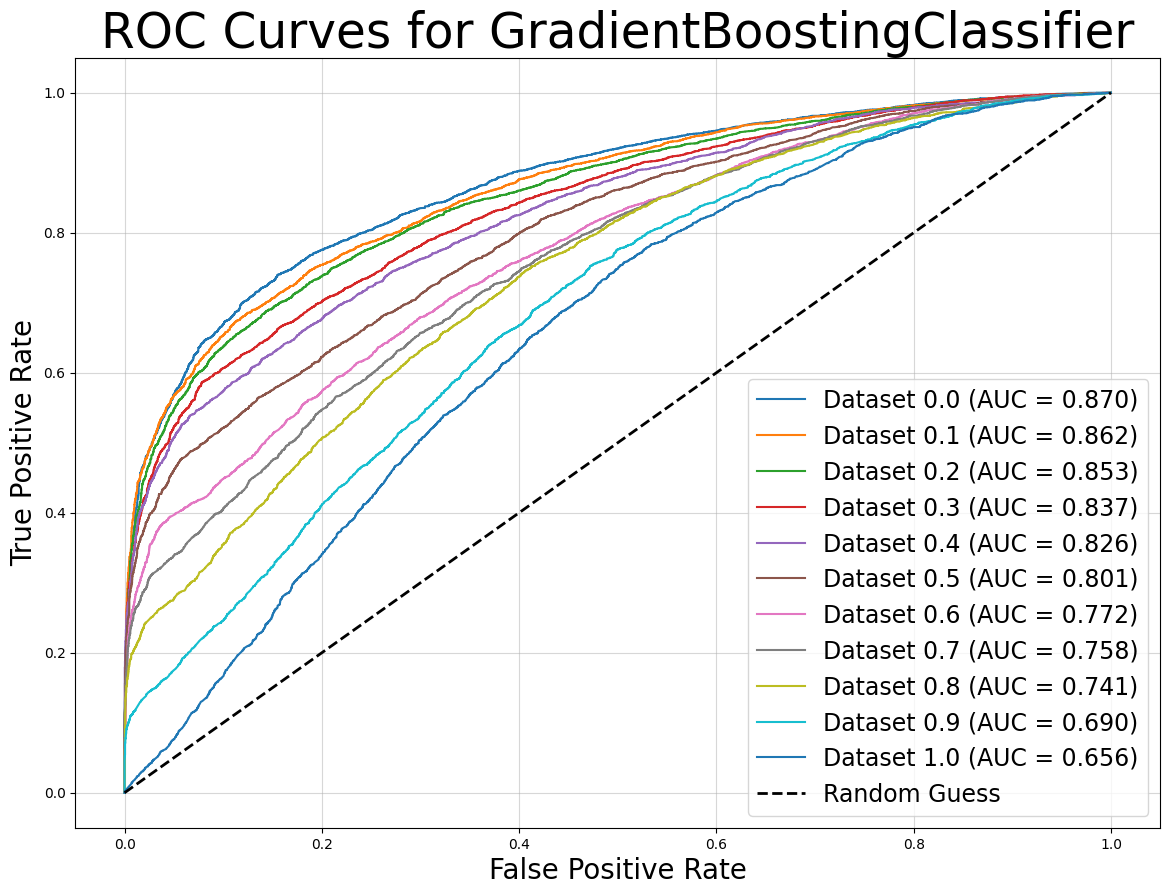
\includegraphics[width=\textwidth]{gbc_auc.png}
                \vskip 0.6em
                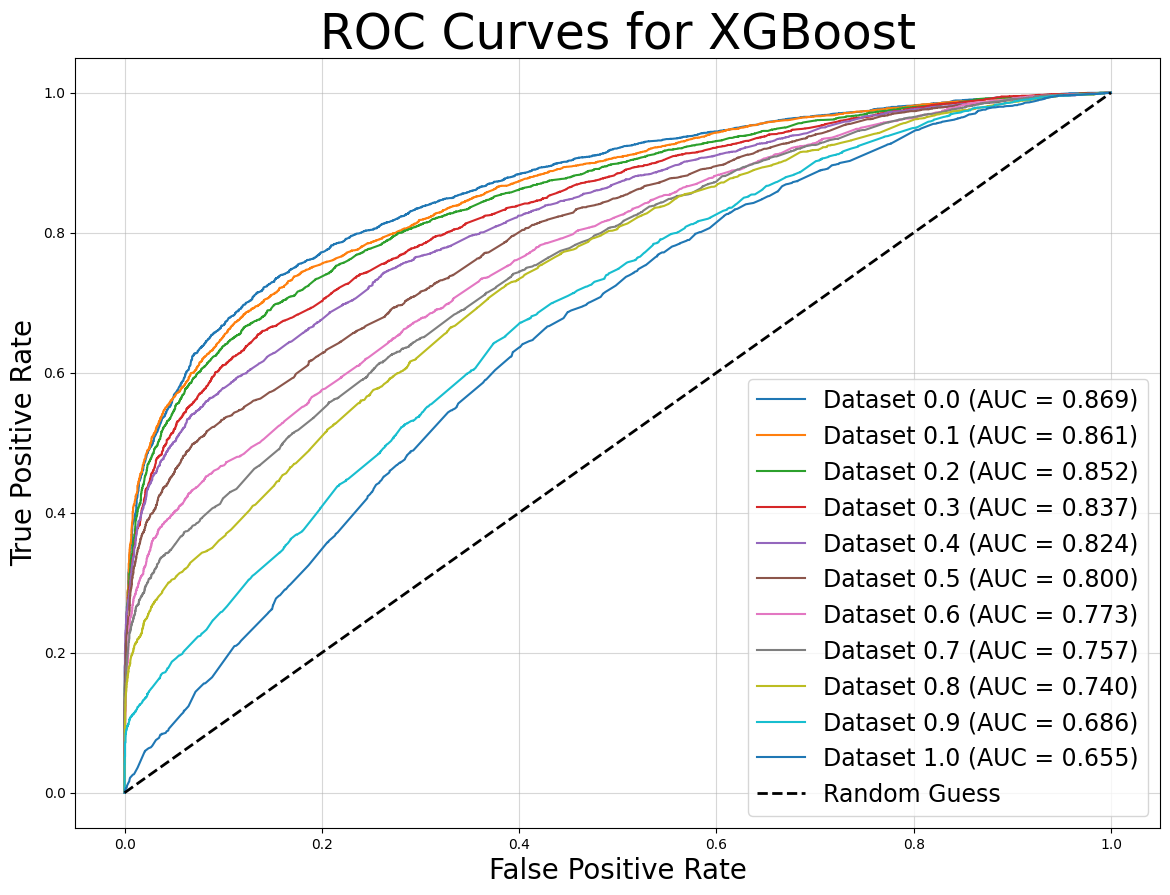
\includegraphics[width=\textwidth]{xgb_auc.png}
            \end{figure}
        \end{column}
    \end{columns}

\end{frame}

\begin{frame}{Performance Comparison}

    \begin{figure}
        \centering
        \vfill
        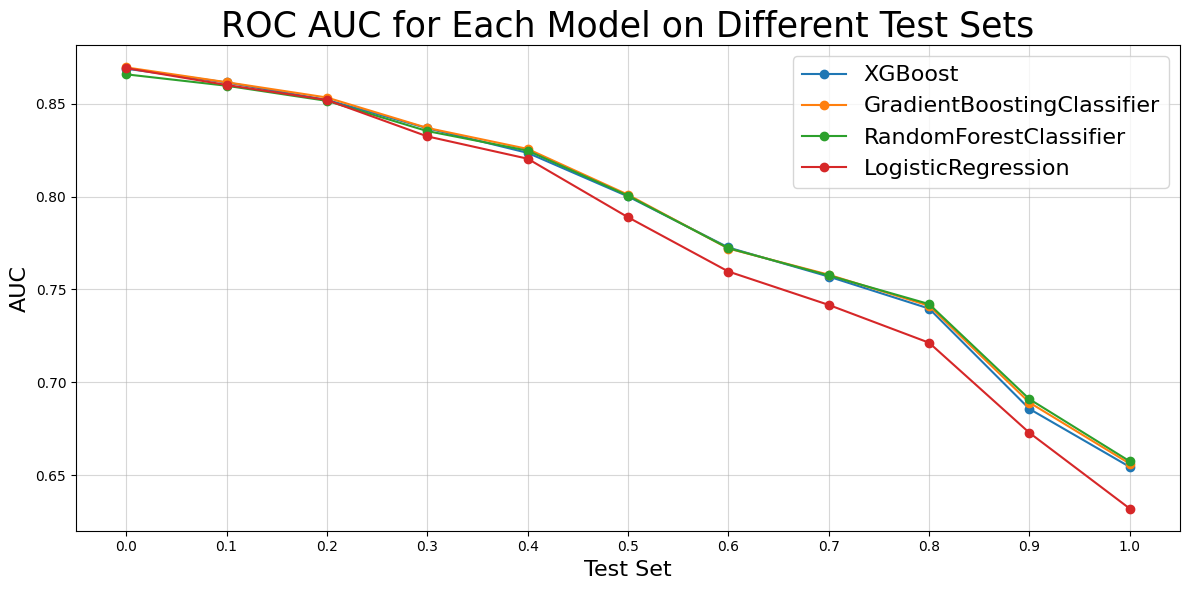
\includegraphics[width=\textwidth]{auc_comp.png}
    \end{figure}

    \small

    The figure illustrates how model performance (AUC) decreases as \ \alpha \ increases, reflecting greater covariate shift.

    Ensemble models demonstrate higher robustness compared to the Logistic Regression baseline.

\end{frame}

\begin{frame}{Statistical Performance Comparison}

    To give statistical support to our study we repeated this experiment $N = 50$ times. Keeping always the same training set (in order to not train the models several times), for each repetition we:
    \begin{enumerate}
        \item defined a new shifted ditribution $\mathcal{N}(\boldsymbol{\mu}_{\text{shift}}, \boldsymbol{\Sigma}_{\text{shift}}) $
        \item created 11 \textbf{testing} datasets $\mathcal{D}_\alpha$ with $\alpha \in \{0.0, 0.1, \ldots, 1.0\}$, where $\alpha$ represents the mixing probability as before
        \item computed the ROC-AUC score for each model on each testing dataset
    \end{enumerate}
\end{frame}

\begin{frame}{Statistical Performance Comparison}

  \begin{figure}
      \centering
      \vfill
      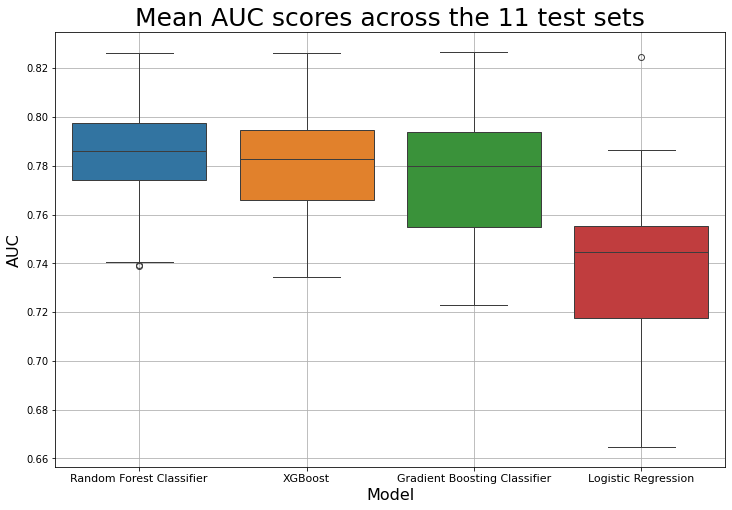
\includegraphics[width=\textwidth]{mean_boxplot.png}
  \end{figure}

\end{frame}

\begin{frame}{Statistical Performance Comparison}

    \begin{figure}
        \centering
        \vfill
        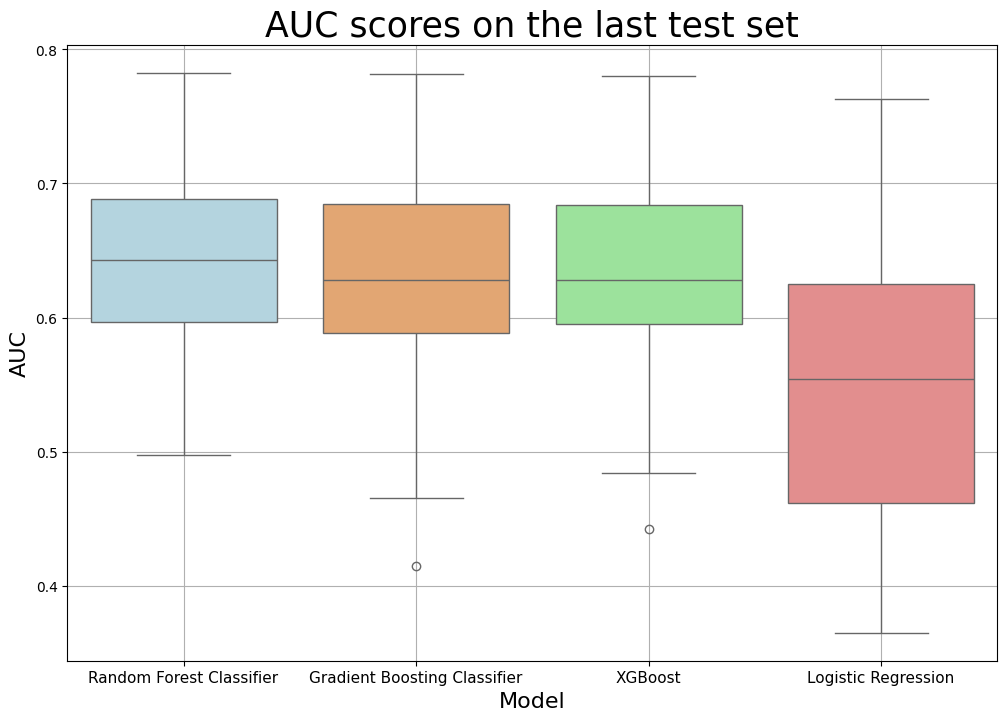
\includegraphics[width=\textwidth]{boxplot.png}
    \end{figure}

\end{frame}
